In order to offer a deployment view of our system, we have decided to use the Deployment Diagram. This choice is due to the fact that this diagram is strictly related to the Component Diagram: indeed, it shows how software components, previously described in the Component Diagram, are deployed in hardware. 

\begin{figure}[H]
        \centering
        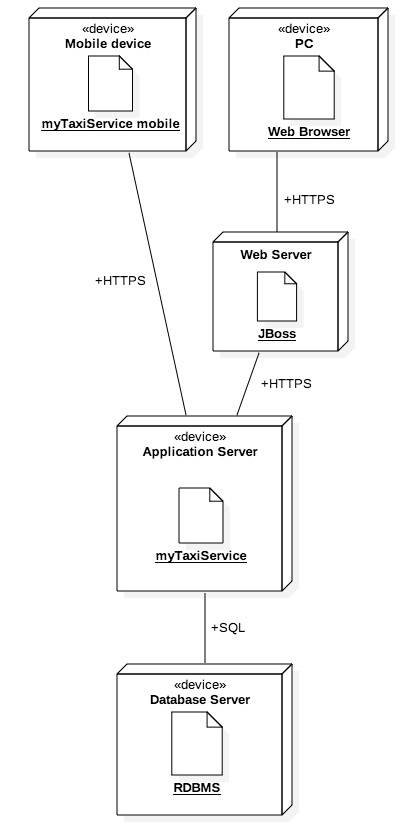
\includegraphics[width=10cm]{./Images/DeploymentDiagram1.png}
        \caption{Deployment Diagram}
\end{figure}

We also give a brief description of the hardware infrastructure. 
\newline
We decided for a dual host configuration: this means that the web server and the application server will be placed on the same machine, while the database will reside on another host. This choice has been preferred to the single host configuration because we want to assure that the data stored in the database are well protected and so, by separating into two hosts, we can put a firewall between them in order to offer an higher security. 
\newline
Our system will have another firewall in order to filter packets coming from the external network and so it will be place before the DMZ to protect the internal network.

\begin{figure}[H]
        \centering
        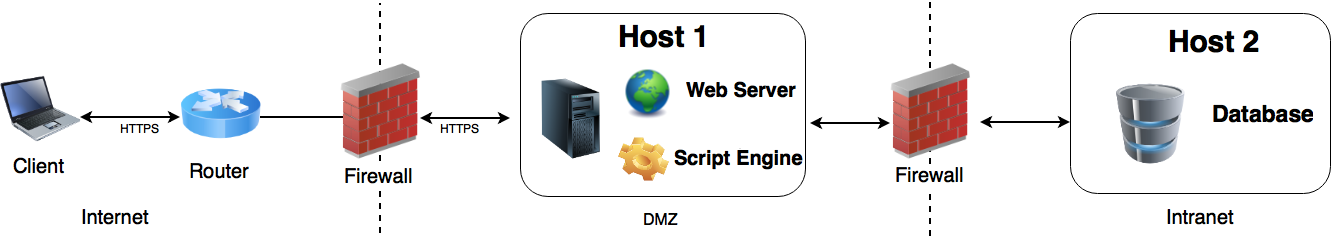
\includegraphics[width=14cm]{./Images/HardwareArchitecture.png}
        \caption{Hardware architecture}
\end{figure}